% !TEX root = ../Ausarbeitung.tex
\section{Containertechnologien} 
\label{sec:Containertechnologien}

In der Geschichte der Containertechnologie traten verschiedene Implementierungsformen auf.
Hierbei waren die ersten Umsetzungen noch sehr einfach aufgebaut und wurden mit den Anforderungen an die Containerdienste immer komplexer.
Im Folgenden findet sich eine Übersicht über die wichtigsten Technologien der Containerisierung.

\begin{figure}[H]
	\begin{center}
		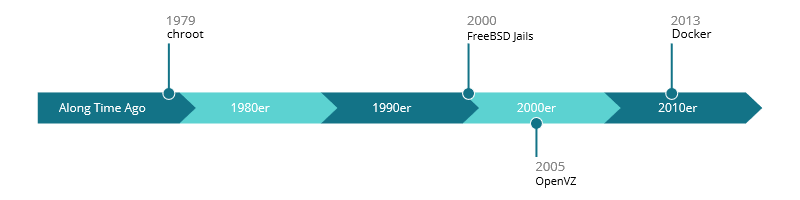
\includegraphics[width=1\textwidth]{ZeitContainer.png}
	\end{center}
	\caption[Containertechnologie im Laufe der Zeit]{Containertechnologie im Laufe der Zeit}
	\label{fig:CTZeit}
\end{figure}


\subsection*{chroot}
\label{sec:chroot}

Chroot ist ein Befehl, der schon früh in Unix-Systemen eingebaut wurde.
Er ermöglicht es, einem Prozess ein anderes Rootverzeichnis zu geben.
Wird in einem Programm \code{chroot()} aufgerufen, wechselt es das Verzeichnis und kann nicht auf Dateien außerhalb der zugewiesenen Struktur zugreifen.
Diese Abschottung eines Prozesses war nie als Sicherheitsfeature vorgesehen und wird hauptsächlich zur Virtualisierung eingesetzt.
Mit dem Befehl können einzelne Prozesse auf Dateiebene von anderen Anwendungen getrennt werden, weitere Sicherheitsmechanismen oder Isolierungen gibt es nicht. \citep{IEEE7830207,569694, MANPAGE01}
\newpage
\subsection*{OpenVZ}
\label{sec:OpenVZ}

\begin{wrapfigure}{l}{0.4\textwidth}
	\vspace{-40pt}
	\begin{center}
		
\includegraphics[width=0.3\textwidth]{openvz.png}
	\end{center}
	\vspace{-15pt}
	\caption[Logo OpenVZ]{Logo OpenVZ \footnotemark}
	\label{fig:openvz}
	\vspace{-30pt}
\end{wrapfigure}
\quellefoot{https://upload.wikimedia.org/wikipedia/commons/b/bb/OpenVZ-logo.png?download}

Im Jahr 2005 veröffentlichte die Firma SWsoft (später umbenannt zu Parallels) ihr Projekt OpenVZ unter der GNU GPL Lizenz. OpenVZ basierte auf der Idee der Container, ermöglicht es jedoch in jedem Container eine eigene Linux-Distribution auszuführen.
Die durch die Containerumgebung abgegrenzten Betriebssysteme teilen sich einen Kernel. Dadurch ist der Overhead von OpenVZ deutlich geringer als bei der klassischen Vollvirtualisierung eines Betriebssystems.
In den einzelnen Containern gibt es jeweils einen eigenen root-User und eine eigene Dateistruktur.
Sie können unabhängig voneinander gestartet und gestoppt werden.
Da sich die Betriebssysteme einen Kernel teilen, müssen die Gastsysteme ebenfalls Linux-Systeme sein.
Da viele der Änderungen von OpenVZ den Linux Kernel betreffen, werden regelmäßig Änderungen von OpenVZ-Patches in diesen übernommen. \citep{OpenVzNews, IEEE4803091,OpenVzHist}


\subsection*{FreeBSD Jails}
\label{sec:jails}
Mit der Veröffentlichung von FreeBSD 4.0 im Jahr 2000 war FreeBSD Jails das erste richtige System für Containervirtualisierung.
Die FreeBSD Jails basieren auf dem Konzept von chroot. Auch hier wird das root-Verzeichnis eines Prozesses geändert. Zusätzlich verbessert Jails das Konzept um einige Aspekte.Jede Jail erhält einen eigenen Hostnamen	und eine eigene IP-Adresse. Sie hat auch ihre eigenen Benutzer, inklusive einem root-Benutzer. \citep{FreeBSDHB14} Durch diese Prozessisolation ergibt sich eine Art Containersystem. Da die Jails als eigener Prozess laufen, können sie unabhängig voneinander gestartet und gestoppt werden.  Jails wird gerne für den Einsatz in Netzwerkaufgaben eingesetzt, da die Performance sehr gut ist. Allerdings besitzt Jails kein so großes Ökosystem wie beispielsweise Docker oder OpenVZ. Daher wird es in der Containervirtualisierung von diesen Gegenspielern verdrängt.


\subsection*{\ac{LXC}}
\label{sec:LXC}
\begin{wrapfigure}{r}{0.4\textwidth}
	\vspace{-40pt}
	\begin{center}
		\includegraphics[width=0.3\textwidth]{LXC.png}
	\end{center}
	\vspace{-15pt}
	\caption[Logo \ac{LXC}]{Logo \ac{LXC} \footnotemark}
	\label{fig:LXC}
	\vspace{-30pt}
\end{wrapfigure}
\quellefoot{https://upload.wikimedia.org/wikipedia/commons/4/40/Linux_Containers_logo.png?download}
\ac{LXC} ist seit der erstmaligen Veröffentlichung 2008 ein offizielles Kernelfeature und in den meisten Distributionen von Linux enthalten. \ac{LXC} ist eine User Space-Schnittstelle für die Erstellung von isolierten Umgebungen innerhalb eines Systems. Dies geschieht durch die Nutzung von Kernel namespaces, Apparmor und SELinux-Profilen sowie chroots und cgroups. Diese Features standen schon vor \ac{LXC} zur Verfügung, jedoch vereinigte sie \ac{LXC} zu einer Schnittstelle für die Erzeugung von Containern. Zu Beginn der Entwicklung von \ac{LXC} war die Isolation der Container nicht gut, sondern glich eher einer Abwandlung der chroot-Funktion. Mit der Zeit wurde die Abschottung jedoch immer besser und die \ac{LXC}-Container wurden zu richtigen virtualisierten Umgebungen. Dies geschah unter anderem dadurch, dass ab Version 1.0 die einzelnen Container als unpriviliegierte Benutzer ausgeführt werden können. Zuvor war dies nicht möglich und eine Abgrenzung der Container nur bedingt gegeben. \ac{LXC} ist eine Technologie, die von vielen weiteren Projekten eingesetzt wird, unter anderem von Proxmox oder Docker (bis Version 1.1)\citep{IEEE7036275, IEEE7185212, IEEE7571957,IEEE7929714,LXCHomepage}


\subsection*{LXD}
\label{sec:lxd}

Um die Verwendung von \ac{LXC} zu vereinfachen, wurde das Tool LXD entwickelt. Es besteht aus drei Elementen: Einem Daemon, der eine REST-API zur Verfügung stellt, einem Befehlszeilenclient sowie einem Open-Stack Nova Plugin. Die vom Daemon bereitgestellte Schnittstelle ermöglicht es, über das Netzwerk auf das Management der Container zuzugreifen. LXD ist somit eine Erweiterung, die eine Schnittstelle zu \ac{LXC}-Containern schafft. Über das Nova Plugin können die einzelnen LXD-Maschinen als Rechenknoten verwendet werden. \citep{LXDHomepage}

\subsection*{Solaris Containers}
\label{sec:solariscontainer}

Im Jahr 2004 veröffentlichte Oracle im Build 51 von Solaris 10 zum ersten Mal ein Feature mit dem Namen Solaris Containers. Solaris Containers stellt eine Technologie dar, mit der auf x86 und SPARC-Systemen Betriebssystemlevelvirtualisierung durchgeführt werden kann. Später zusammengelegt zu Solaris Zones, bestanden die beiden Technologien Solaris Containers und Solaris Zones parallel zueinander. Dabei war Zones eine klassische Virtualisierungsplattform mit Hypervisor und Containers eine Containertechnologie, die analog zu chroot funktionierte. Mit der Zusammenlegung von Containers und Zones zum neuen Zones wurde daraus eine Containerumgebung, in der die Container sicher voneinander und dem Host getrennt sind und von einem Resourcenmanagement kontrolliert werden. \citep{OracleZonesIntro,OracleZonesOver}
	

%\subsection{Windows Containers}
%s\label{sec:WindowsContainers}



\subsection*{Docker}
\label{sec:Docker}


dotCloud veröffentlichte im März 2013 das Projekt mit dem Namen Docker, dieses Projekt stellte Solomon Hykes auf der PyCon 2013 zum ersten Mal der Öffentlichkeit vor. \citep{dockeryout1} Ein paar Monate später kündigte dotCloud Inc. an, den Firmennamen zu Docker Inc. zu ändern und sich hauptsächlich der Entwicklung des Docker Ökosystems zu widmen. \citep{dockerblog} Die Firma Docker Inc. (im Folgenden "`Docker Inc."' oder "`Hersteller"') hat bis zum heutigen Tag das Projekt Docker (im Folgenden "`Docker"') weiterentwickelt und das zugehörige Ökosystem ausgebaut. So wurde unter anderem der DockerHub eingerichtet, eine Plattform um Images zu teilen und auszutauschen. \citep{dockermanual}

Zu Beginn war Docker lediglich eine Werkzeugsammlung um \ac{LXC}-Container zu verwalten. Jedoch baute Docker Inc. diese Sammlung immer weiter aus und erweiterte das System um Funktionen, die vom unterliegenden Linux-Betriebssystem nicht gegeben waren. Mit der Version 0.9 veröffentlichte Docker Inc. den neuen Treiber libcontainer und nutzte ihn ab diesem Zeitpunkt als native Umgebung für Docker-Container. \citep{dockerblog2} Zu Beginn unterstützte Docker lediglich Linux-Container und nutzte dazu unter Windows eine virtuelle Maschine (Windows 7 \& 8) oder das Linux-Subsystem (Windows 10). Ab der Version 17.11 von Docker für Windows und dem Windows 10 Fall Creators Update konnten erstmals Windows Container genutzt werden. \citep{dockerblogwin} Auch entwickelte Docker Inc. weitere Zwischebenen, um sich von \ac{LXC} zu lösen und die Umgebung in Module zu teilen. So entstand containerd, ein Container-Daemon, mit dem die Docker Engine kommuniziert. Dieser Daemon wiederum kann mit einem OCI-konformen Container-Tool umgehen und über dieses Container starten. Ein solches Tool ist das eigene runC. Auf diese Art können Docker-Container auch durch andere Orchestrierungstools wie Kubernetes oder Swarm verwaltet werden (\Vgl \Abschnitt{Cluster}). \citep{Buch}

Zum heutigen Zeitpunkt ist Docker die führende Containerumgebung (\Vgl \Abbildung{Stats2}), daher wird die Funktion derselben im Folgenden anhand eines Beispielcontainers aufgezeigt:

In diesem Beispiel soll innerhalb eines Docker-Containers ein Python-Skript ausgeführt werden. Als Basis für eine Container-Instanz dient ein schreibgeschütztes Image. Dieses enthält alle benötigten Teile des OS abgesehen vom Kernel, denn dieser wird bereits durch den Host zur Verfügung gestellt. Zusätzlich gehören auch benötigte Abhängigkeiten zu einem Image. Auf diesem schreibgeschützten Teil wird dann ein schreibbarer Layer aufgebaut, wenn von dem Image eine Container-Instanz abgeleitet wird. Wird die Container-Instanz beendet, sind alle Änderung innerhalb des schreibbaren Layer verloren. Um die Änderungen zu sichern, kann ein sogenannter Snapshot angelegt werden, der dem Image einen weiteren read-only-Layer hinzufügt. Die Anzahl der Layer ist, je nach Docker-Version, auf 127 beschränkt. \citep{Buch, dockermanual} \newpage Der Aufbau des Images unseres Beispielcontainers sieht aus wie in \Abbildung{docker1} dargestellt:

\begin{figure}[h]
    \begin{center}
        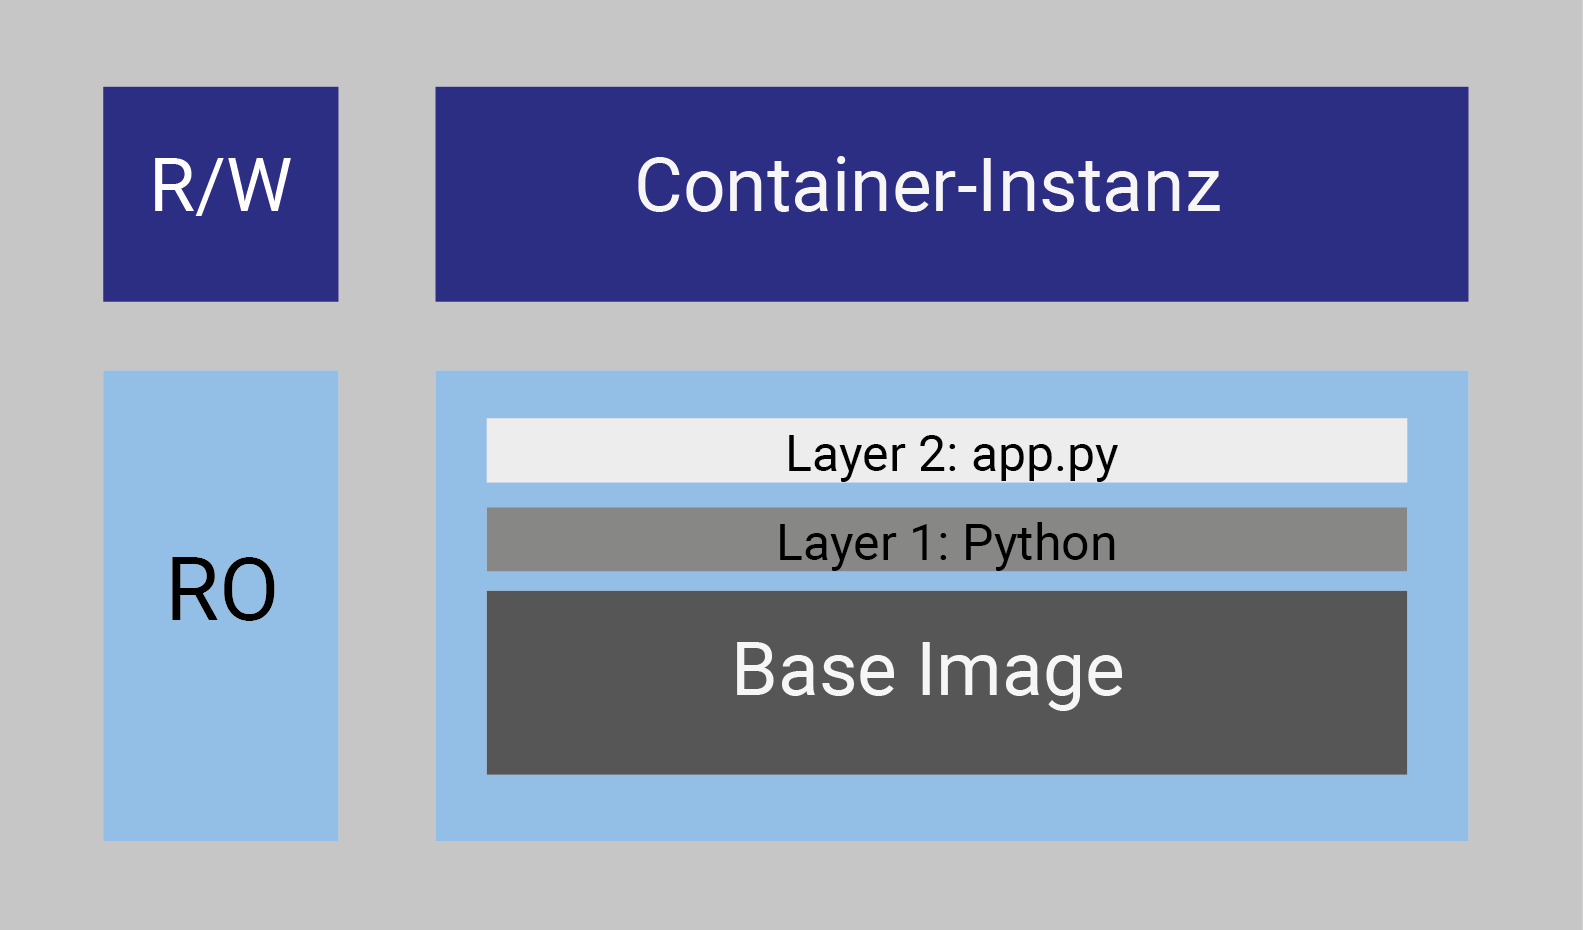
\includegraphics[width=0.6\textwidth]{DockerImage.png}
    \end{center}
    \caption[Image des Beispielcontainer ]{Image des Beispielcontainer}
    \label{fig:docker1}
    \end{figure}

Als Basis dient ein Image, in dem Alpine Linux installiert ist. Python wird als weiterer Layer hinzugefügt. Zu diesen Layern wird noch das Python-Skript hinzugefügt. Dies zusammen ergibt dann den schreibgeschützten Teil, von dem die Container-Instanz abgeleitet wird. In dieser legt das Python-Skript Dateien an und schreibt in diese. Wird der Container beendet, werden alle angelegten Dateien verworfen.\\
Der Aufbau des Images kann in einem Dockerfile beschrieben werden. Für unser Beispiel sieht dieses wie folgt aus:

\begin{lstlisting}[language=docker,caption={Dockerfile},label={code:dockerfile}]
FROM python:3 

WORKDIR /usr/src/app

COPY ./app.py ./app.py

CMD ["python", "./app.py"]
\end{lstlisting}

In dem Dockerfile wird zuerst definiert, dass das Image auf dem vorhanden Python-Image aufbauen soll. Dieses wiederum baut auf einem Alpine-Linux-Image auf. Daraufhin wird das aktuelle Arbeitsverzeichnis im Container geändert. Anschließend wird die im Arbeitsverzeichnis des Host abgelegte Datei "`app.py"' in das Arbeitsverzeichnis des Container übertragen und schließlich der Befehl definiert, der beim Start des Containers ausgeführt werden soll. Das Python-Skript legt eine Datei an und gibt deren Dateiname und Inhalt in der Konsole aus:
\begin{lstlisting}[language=python,caption={app.py},label={code:pythonapp}]
#!/usr/bin/python3

print("Ausgabe zur Kommandozeile")
file=open("datei.txt", "a+")
print("Dateiname: ", file.name)
file.write("Eine neue Zeile")
file.close()
print(open("datei.txt","r").read())
\end{lstlisting}
Nun kann mit dem Befehl \code{docker build} das Image erstellt werden. Dabei lädt Docker zunächst das Image von python aus dem oben genanten Docker-Hub herunter und legt darauf den Layer mit dem Python-Skript:

\begin{lstlisting}[language=bash,caption={Terminalausgabe docker build},label={code:dockerbuild}]
user@dockerpc:~$ docker build -t pythontest .
Sending build context to Docker daemon 311.4MB
Step 1/4 : FROM python:3
 ---> 638817465c7d
Step 2/4 : WORKDIR /usr/src/app
---> 8d3ab23442c9
Step 3/4 : COPY ./app.py ./app.py
---> 2b0882cadee4
Step 4/4 :  CMD ["python", "./app.py"]
---> 5a8a392a0856
Successfully built 5a8a392a0856
Successfully tagged pythontest:latest
\end{lstlisting}

Nun liegt das Image bereit und es kann ein Container davon abgeleitet werden. Dazu reicht der einfache Befehl \code{docker run}, um den Container zu starten:

\begin{lstlisting}[language=bash,caption={Terminalausgabe docker run},label={code:dockerbuild}]
user@dockerpc:~$ docker run pythontest
Ausgabe zur Kommandozeile
Dateiname: datei.txt
Eine neue Zeile
\end{lstlisting}

Hier wird nun das Python-Skript in dem Container ausgeführt und der Container daraufhin beendet und somit auch die beschriebene Datei gelöscht. Wird der Container erneut ausgeführt, so wird eine neue Datei erstellt:

\begin{lstlisting}[language=bash,caption={Terminalausgabe docker run mehrfach},label={code:dockerbuild}]
user@dockerpc:~$ docker run pythontest
Ausgabe zur Kommandozeile
Dateiname: datei.txt
Eine neue Zeile

user@dockerpc:~$ docker run pythontest
Ausgabe zur Kommandozeile
Dateiname: datei.txt
Eine neue Zeile
\end{lstlisting}

Die Layer, aus denen Docker die verschiedenen Images aufbaut wurden von Docker Inc. in den ursprünglichen \ac{LXC}-Container hinzugefügt und später zum hauseigenen libcontainer übernommen. Durch diese Layer ist es einfacher Ressourcen zu teilen. Wenn mehrere Images auf Python oder Alpine-Linux aufbauen sollen, so müssen diese beiden Ressourcen nicht mehrfach heruntergeladen werden, sondern stehen jedem Image zur Verfügung. Dies ist einer der Gründe, warum Docker nach der Veröffentlichung große Popularität erreichte und heute die führende Containertechnologie ist. \citep{dockermilestones}



\subsection*{rkt}
\label{sec:rkt}

\begin{wrapfigure}{l}{0.4\textwidth}
	\vspace{-40pt}
	\begin{center}
		
\includegraphics[width=0.3\textwidth]{rkt.png}
	\end{center}
	\vspace{-15pt}
	\caption[Logo rkt]{ \footnotemark}
	\label{fig:rkt}
	\vspace{-30pt}
\end{wrapfigure}
\quellefoot{https://github.com/rkt/rkt/raw/master/logos/rkt-horizontal-color.png}


rkt (Ausprache wie "rocket") ist eine Containerengine, die sich als Alternative zu Docker etabliert hat und von CoreOS veröffentlicht wurde und weiterentwickelt wird. Das Projekt ist ein Open-Source-Projekt und unter der Apache License 2.0 veröffentlicht. \citep{RepoRkt} Unter rkt werden viele Grundgedanken von UNIX umgesetzt. Z.B. liegen alle Container als Dateien vor, die einfach verwaltet werden können. Auch legt rkt einen großen Wert auf Sicherheit und setzt dazu verschiedene Techniken ein, die inzwischen von den meisten Konkurennten übernommen wurden. So kann rkt für jeden Container entscheiden, ob dieser auf Basis von KVM oder einer virtuellen Maschine isoliert wird und führt alle Prozesse, auch den Download von Images, als nicht priviligierter Benutzer aus. In rkt wird die kleinste Einheit Pod genannt. Sie kann aus einem oder mehreren Containeren bestehen, welche sich die Ressourcen teilen. So passt das Konzept von  rkt direkt zu den Konzepten von  Cluster-Managern. Auch besitzt rkt keinen zentralen Service, der alle Container überwacht, sondern arbeitet direkt mit dem systemeigenen systemd zusammen, um die Container zu verwalten. Somit lässt sich rkt auch direkt mit Kubernetes verknüpfen, für das der Herausgeber von rkt, CoreOS, die kommerzielle Implementierung Tectonic entwickelt. rkt unterstützt auch die Konvertierung von Docker-Containern zu rkt-Pods. \citep{HomepageRkt,ixrkt}

